\chapter{Text classification} \label{chapt1}

\section{Relevance of the problem} \label{sect1_1}

Nowadays, retail e-commerce sales are quickly expanding. A large online e-commerce
websites serve millions of users’ requests per day. Therefore it necessary to make the process of registrations and purchases as much convenient and fast as possible. For many classifieds platform such as Amazon or Avito users who would like to create a new advertisement must to fulfill compulsory fields: title, description, price and category. Choosing category can be a tricky moment, because in most cases users have a choice more then from three hundreds categories. Therefore, the problem  of advertisement automatic category prediction is very important in terms to save moderators' time and as a result decrease number of necessary moderators to process them. The effective algorithm which would work with text data, have a high accuracy and an appropriate speed are in high demand.
%In this paper I want to consider models that are used for texts classification and pay the special attention for Deep Learning approaches.  

\section{Statement of classification problem} \label{sect1_2}


Classification problem - the problem of identifying to which category a new observation belongs. The basic example can be situation when you receive a new email and algorithm automatically decides whether it belongs to social network, promotions or business letters.


\newcommand{\docsetlabeled}{\mathbb{D}}

In text classification, we are given a description  $d \in \mathbb{X}$ of a document, where $\mathbb{X}$ is the document space ; and a fixed set of classes  $\mathbb{C} = \{ c_1,c_2,\ldots,c_J \}$. Classes are also called categories or labels . Typically, the document space  $\mathbb{X}$ is some type of high-dimensional space, and the classes are human defined for the needs of an application, as in the examples China and documents that talk about multicore computer chips above. We are given a training set  $\docsetlabeled$ of labeled documents  $d $, where  $d \in \mathbb{X} \times \mathbb{C}$. For example: 

\begin{equation}
\label{eq:equation3}
\langle\mbox{d, c}\rangle=\langle\mbox{Beijing joins the World Trade Organization}, \emph{China}\rangle
\end{equation}

for the one-sentence document Beijing joins the World Trade Organization and the class (or label) China.
Using a learning method or learning algorithm , we then wish to learn a classifier or classification function  $\gamma $ that maps documents to classes:

\begin{equation}
\label{eq:equation4}
\gamma: \mathbb{X} \rightarrow \mathbb{C}
\end{equation}

This type of learning is called supervised learning because a supervisor (the human who defines the classes and labels training documents) serves as a teacher directing the learning process. We denote the supervised learning method by $\Gamma$ and write  $\Gamma(\docsetlabeled) = \gamma$. The learning method $\Gamma$ takes the training set  $\docsetlabeled$ as input and returns the learned classification function $\gamma $.

The classes in text classification often have some interesting structure such as the hierarchy in Figure ~\ref{img:hierarchy} . There are two instances each of region categories, industry categories, and subject area categories. A hierarchy can be an important aid in solving a classification problem. Our goal in text classification is high accuracy on test data or new data - for example, the newswire articles that we will encounter tomorrow morning in the multicore chip example. It is easy to achieve high accuracy on the training set (e.g., we can simply memorize the labels). But high accuracy on the training set in general does not mean that the classifier will work well on new data in an application. When we use the training set to learn a classifier for test data, we make the assumption that training data and test data are similar or from the same distribution.\cite[p.256-257]{manning}

\begin{figure}[ht] 
	\center
	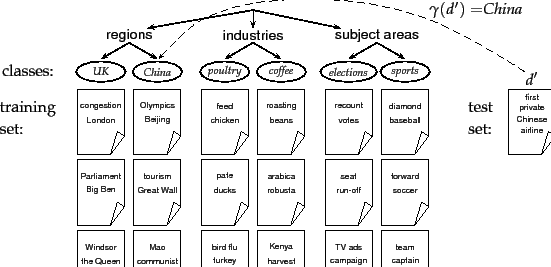
\includegraphics [scale=0.6] {hierarchy}
	\caption{Classes, training set, and test set in text classification.} 
	\label{img:hierarchy}  
\end{figure}


\section{Short review of existing mathematical models, which can be used to solve the classification problem} \label{sect1_3}

\begin{figure}[ht] 
	\center
	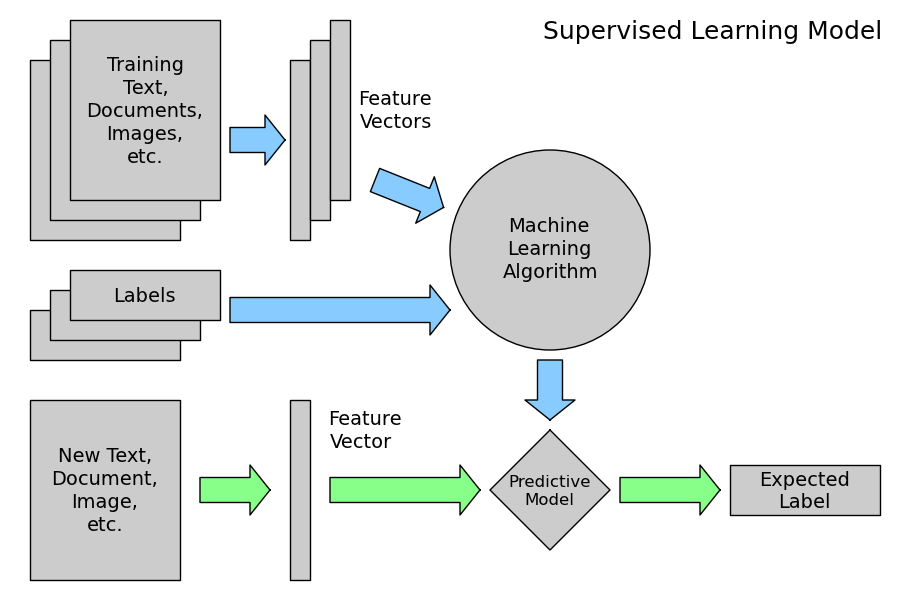
\includegraphics [scale=0.6] {work_flow}
	\caption{Supervised learning work flow.} 
	\label{img:supervised_learning_work_flow}  
\end{figure}

Supervised learning - the machine learning task of inferring a function from labeled training data. The training data consist of a set of training examples. Between inputs and reference outputs there may be some dependence, but it is unknown. On the basis of this data, it is necessary to restore the dependence. In order to measure the accuracy a quality function can be introduced.\cite[p.7]{foundationsml} The diagram of the supervised learning process in presented in Figure ~\ref{img:supervised_learning_work_flow} 
\\

\noindent \textbf{Here are some of the most important supervised learning algorithms}:
\begin{enumerate}
	\item Naive Bayes .\cite{NB1}.\cite{NB2}
	%\item k-Nearest Neighbors
	\item Logistic Regression .\cite{LR}
	\item Support Vector Machines (SVMs) .\cite{svm}
	\item Decision Trees and Random Forests .\cite{manning}
	\item Neural networks .\cite{manning}
\end{enumerate}

1.\textbf{ Naive Bayes} - a probabilistic learning method.
 The probability of a document $d$ being in class $c$ is computed as 
 \begin{equation}
 \label{eq:equation5}
 \displaystyle P(c\vert d) \propto P(c) \prod_{1 \leq k \leq n_d} P(t_k \vert c)
 \end{equation}
 
where  $P(t_k \vert c)$ is the conditional probability of term  $t_k$ occurring in a document of class $c$. We interpret  $P(t_k \vert c)$ as a measure of how much evidence  $t_k$ contributes that $c$ is the correct class. $P(c)$ is the prior probability of a document occurring in class $c$. If a document's terms do not provide clear evidence for one class versus another, we choose the one that has a higher prior probability.  
$\langle t_1,t_2,\ldots,t_{n_d}\rangle$ are the tokens in $d$ that are part of the vocabulary we use for classification and $n_d$ is the number of such tokens in $d$.
\\

In text classification, our goal is to find the best class for the document. The best class in NB classification is the most likely or maximum a posteriori ( MAP ) class $c_{map}$: 

\begin{equation}
\label{eq:equation5}
c_{map} = argmax_{c \in \mathbb{C}} \hat{P}(c \vert d) = argmax_{c \in \mathbb{C}} \hat{P}(c) \prod_{1 \leq k \leq n_d} \hat{P}(t_k \vert c).
\end{equation}

For the priors this estimate is

\begin{equation}
\label{eq:equation6}
\displaystyle \hat{P}(c) = \frac{N_c}{N},
\end{equation}

where $N_c$ is the number of documents in class $c$ and $N$ is the total number of documents.
\\
We estimate the conditional probability  $\hat{P}(t\vert c)$ as the relative frequency of term $t$ in documents belonging to class $c$: 


\begin{equation}
\label{eq:equation7}
\hat{P}(t \vert c) = \frac{T_{ct}+1}{\sum_{t^{'} \in V} (T_{ct^{'}}} + 1),
\end{equation}

where $T_{ct}$ is the number of occurrences of $t$ in training documents from class $c$, including multiple occurrences of a term in a document
$T_{ct}$ is a count of occurrences in all positions $k$ in the documents in the training set,
$V$ - vocabulary
To eliminate zeros, we use add-one or Laplace smoothing, which simply adds one to each count.\cite[p.258-260]{manning}

\begin{figure}[ht] 
	\center
	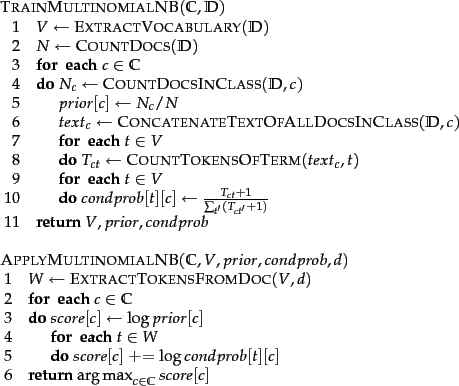
\includegraphics [scale=0.7] {NB_algorithm}
	\caption{Naive Bayes algorithm (multinomial model): Training and testing.} 
	\label{img:NB_algorithm}  
\end{figure}

2.\textbf{Logistic Regression}.
For now, we will focus on the binary classification problem in which y can take on only two values, 0 and 1


